% Created 2024-06-05 mié 17:24
% Intended LaTeX compiler: pdflatex
\documentclass[presentation]{beamer}
\usepackage[utf8]{inputenc}
\usepackage[T1]{fontenc}
\usepackage{graphicx}
\usepackage{grffile}
\usepackage{longtable}
\usepackage{wrapfig}
\usepackage{rotating}
\usepackage[normalem]{ulem}
\usepackage{amsmath}
\usepackage{textcomp}
\usepackage{amssymb}
\usepackage{capt-of}
\usepackage{hyperref}
\usetheme{Madrid}
\usecolortheme{}
\usefonttheme{}
\useinnertheme{}
\useoutertheme{}
\author{Luis Enrique Perez Señalin}
\date{\textit{<2024-06-05 mié>}}
\title{Taller Aritmética Digital y Lógica Digital 1}

\hypersetup{
 pdfauthor={Luis Enrique Perez Señalin},
 pdftitle={Taller Aritmética Digital y Lógica Digital 1},
 pdfkeywords={},
 pdfsubject={},
 pdfcreator={Emacs 27.1 (Org mode 9.3)}, 
 pdflang={Spanish}}
\begin{document}

\maketitle
\begin{frame}{Outline}
\tableofcontents
\end{frame}


\section{Ejercicios}
\label{sec:org7a90f67}
\begin{frame}[label={sec:org582d926}]{presentacion 1}
\begin{center}
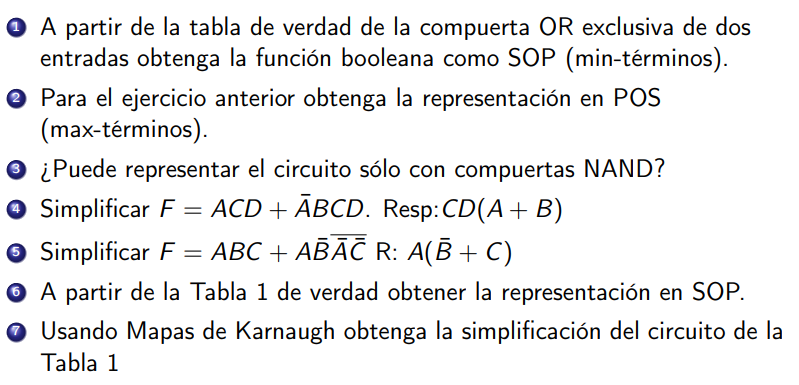
\includegraphics[width=.9\linewidth]{./enunciado1.png}
\end{center}
\end{frame}


\section{Respuestas}
\label{sec:org764525b}
\begin{frame}[label={sec:orgec27021}]{presentacion 2}
Ejercicio 1
\begin{center}
\begin{tabular}{|l|l|l|}
\hline
x1 & x2 & x1(+)x2 \\
\hline
0 & 0 & 0 \\
\hline
0 & 1 & 1 \\
\hline
1 & 0 & 1 \\
\hline
1 & 1 & 0 \\
\hline
\end{tabular}
\end{center}
SOP 
$$(\bar{x1}*x2)+(x1*\bar{x2})$$
\end{frame}
\begin{frame}[label={sec:org7146b5c}]{Presentacion3}
Ejercicio2
POS
$$F(x1,x2) = (x1+x2) * (\bar{x1}+\bar{x2})$$
\end{frame}

\begin{frame}[label={sec:org49b4636}]{Presentacion4}
Ejercicio3
\begin{center}
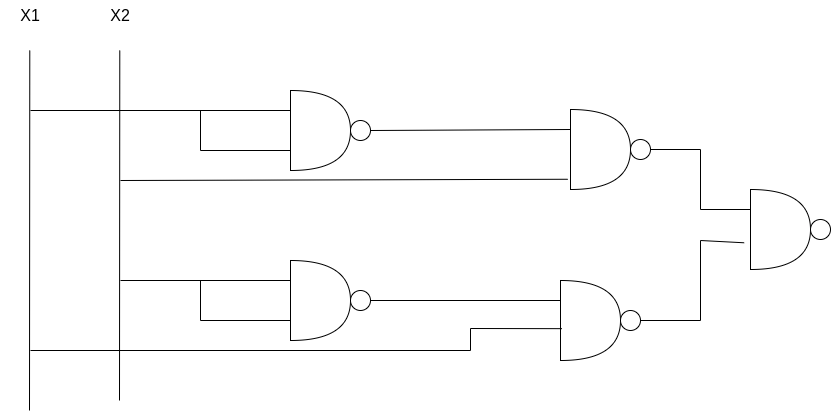
\includegraphics[width=.9\linewidth]{./diagrama.png}
\end{center}
\end{frame}

\begin{frame}[label={sec:org3a0ee33}]{Presentacion5}
Ejercicio4
$$F = ACD + \bar{A}BCD$$
$$  = CD(A+\bar{A}B)  $$
$$  = CD(A+B)         $$
\end{frame}

\begin{frame}[label={sec:org7269555}]{Presentacion6}
Ejercicio5
$$F = ABC + A\bar{B}\overline{\bar{A}\bar{C}}$$                                                        
$$  = ABC + A\bar{B}(\overline{\overline{A + C}})$$                                                        
$$  = ABC + A\bar{B}(A+C)$$
$$  = ABC + A\bar{B} + AC\bar{B}$$
$$  = AC(B + \bar{B}) + A\bar{B}$$
$$  = AC + A\bar{B}$$
$$  = A(C + \bar{B}$$
\end{frame}

\begin{frame}[label={sec:org63ff388}]{Presentacion7}
Ejercicio 6
$$F(x1,x2) = \bar{X1}X2 + X1\bar{X2}$$
\end{frame}

\begin{frame}[label={sec:orge9334e0}]{Presentacion8}
Ejercicio 7
\begin{center}
\begin{tabular}{|l|l|l|l|}
\hline
A & B & C & F \\
\hline
0 & 0 & 0 & 0 \\
\hline
0 & 0 & 1 & 0 \\
\hline
0 & 1 & 0 & 1 \\
\hline
0 & 1 & 1 & 1 \\
\hline
1 & 0 & 0 & 0 \\
\hline
1 & 0 & 1 & 0 \\
\hline
1 & 1 & 0 & 1 \\
\hline
1 & 1 & 1 & 0 \\
\hline
\end{tabular}
\end{center}
\end{frame}

\begin{frame}[label={sec:orgde1e209}]{Presentacion9}
Tabla

\begin{center}
\begin{tabular}{|l|l|l|l|l|}
\hline
A$\backslash$BC & 00 & 01 & 11 & 10 \\
\hline
0 & & & 1 & 1 \\
\hline
1 & & & & 1 \\
\hline
\end{tabular}
\end{center}

$$F = \bar{A}B + B\bar{C}+A\bar{B}C$$
\end{frame}
\end{document}
